% vim: spell spelllang=en_gb
\appendix
\chapter{Diagrams}\label{appendix:raw}
\begin{figure}
\begin{center}
  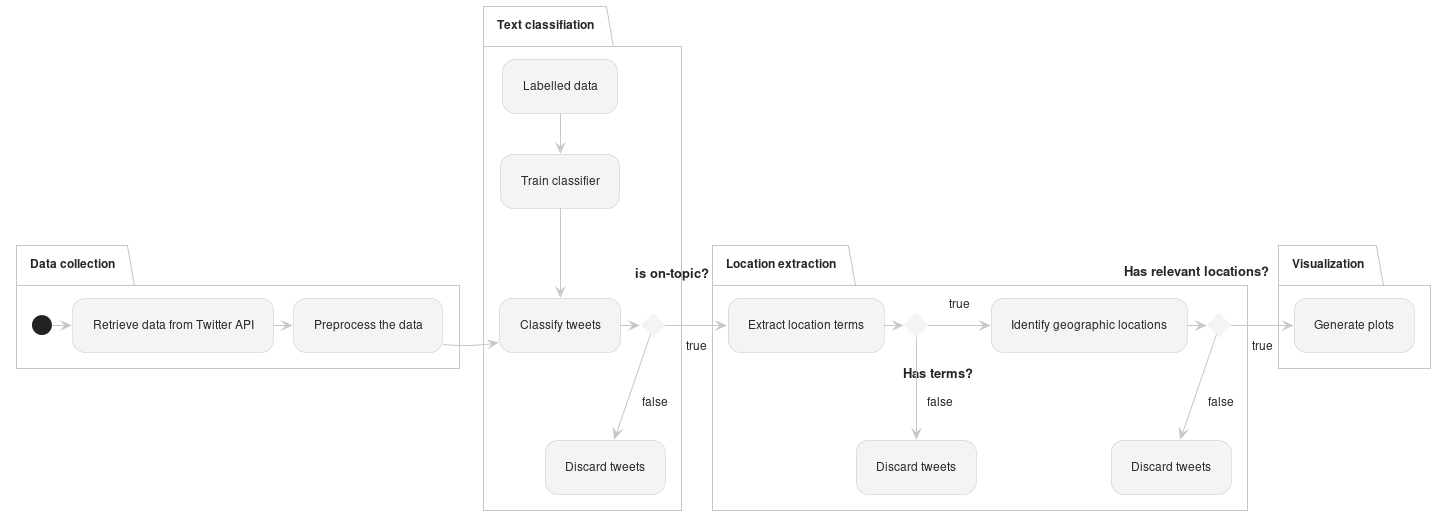
\includegraphics[angle=90, width=\dimexpr\textwidth-11cm\relax, height=\textheight, keepaspectratio]{./images/pipeline.png}
\end{center}
\caption{Flow chart for the pipeline}
\label{fig:flow_chart_big}
\end{figure}
\chapter{Examples}\label{appendix:examples}
\section{Nominatim output example}
 \begin{verbatim}
  {
    "place_id": "100149",
    "licence": "Data © OpenStreetMap contributors, 
                ODbL 1.0. https://osm.org/copyright",
    "osm_type": "node",
    "osm_id": "107775",
    "boundingbox": ["51.3473219", "51.6673219", 
                    "-0.2876474", "0.0323526"],
    "lat": "51.5073219",
    "lon": "-0.1276474",
    "display_name": "London, Greater London, England, 
                     SW1A 2DU, United Kingdom",
    "class": "place",
    "type": "city",
    "importance": 0.9654895765402,
    "icon": "https://nominatim.openstreetmap.org/
             images/mapicons/poi_place_city.p.20.png",
    "address": {
      "city": "London",
      "state_district": "Greater London",
      "state": "England",
      "ISO3166-2-lvl4": "GB-ENG",
      "postcode": "SW1A 2DU",
      "country": "United Kingdom",
      "country_code": "gb"
    },
    "extratags": {
      "capital": "yes",
      "website": "http://www.london.gov.uk",
      "wikidata": "Q84",
      "wikipedia": "en:London",
      "population": "8416535"
    }
  }                           
  \end{verbatim}
                
